%%%%%%%%%%%%%%%%%%%%%%%%%%%%%%%%%%%%%%%%%%%%%%%%%%%%%%%%%%%%%%%%%%%%%%%%%%%%%%%%
%%%%%%%%%%%%%%%%%%%%%%%%%%%%%%%%%%%%%%%%%%%%%%%%%%%%%%%%%%%%%%%%%%%%%%%%%%%%%%%%
%%                                                                            %%
%% thesistemplate.tex version 3.20 (2018/08/31)                               %%
%% The LaTeX template file to be used with the aaltothesis.sty (version 3.20) %%
%% style file.                                                                %%
%% This package requires pdfx.sty v. 1.5.84 (2017/05/18) or newer.            %%
%%                                                                            %%
%% This is licensed under the terms of the MIT license below.                 %%
%%                                                                            %%
%% Written by Luis R.J. Costa.                                                %%
%% Currently developed at the Learning Services of Aalto University School of %%
%% Electrical Engineering by Luis R.J. Costa since May 2017.                  %%
%%                                                                            %%
%% Copyright 2017-2018, by Luis R.J. Costa, luis.costa@aalto.fi,              %%
%% Copyright 2017-2018 Swedish translations in aaltothesis.cls by Elisabeth   %%
%% Nyberg, elisabeth.nyberg@aalto.fi and Henrik Wallén,                       %%
%% henrik.wallen@aalto.fi.                                                    %%
%% Copyright 2017-2018 Finnish documentation in the template opinnatepohja.tex%%
%% by Perttu Puska, perttu.puska@aalto.fi, and Luis R.J. Costa.               %%
%% Copyright 2018 English template thesistemplate.tex by Luis R.J. Costa.     %%
%% Copyright 2018 Swedish template kandidatarbetsbotten.tex by Henrik Wallen. %%
%%                                                                            %%
%% Permission is hereby granted, free of charge, to any person obtaining a    %%
%% copy of this software and associated documentation files (the "Software"), %%
%% to deal in the Software without restriction, including without limitation  %%
%% the rights to use, copy, modify, merge, publish, distribute, sublicense,   %%
%% and/or sell copies of the Software, and to permit persons to whom the      %%
%% Software is furnished to do so, subject to the following conditions:       %%
%% The above copyright notice and this permission notice shall be included in %%
%% all copies or substantial portions of the Software.                        %%
%% THE SOFTWARE IS PROVIDED "AS IS", WITHOUT WARRANTY OF ANY KIND, EXPRESS OR %%
%% IMPLIED, INCLUDING BUT NOT LIMITED TO THE WARRANTIES OF MERCHANTABILITY,   %%
%% FITNESS FOR A PARTICULAR PURPOSE AND NONINFRINGEMENT. IN NO EVENT SHALL    %%
%% THE AUTHORS OR COPYRIGHT HOLDERS BE LIABLE FOR ANY CLAIM, DAMAGES OR OTHER %%
%% LIABILITY, WHETHER IN AN ACTION OF CONTRACT, TORT OR OTHERWISE, ARISING    %%
%% FROM, OUT OF OR IN CONNECTION WITH THE SOFTWARE OR THE USE OR OTHER        %%
%% DEALINGS IN THE SOFTWARE.                                                  %%
%%                                                                            %%
%%                                                                            %%
%%%%%%%%%%%%%%%%%%%%%%%%%%%%%%%%%%%%%%%%%%%%%%%%%%%%%%%%%%%%%%%%%%%%%%%%%%%%%%%%
%%                                                                            %%
%%                                                                            %%
%% An example for writting your thesis using LaTeX                            %%
%% Original version and development work by Luis Costa, changes to the text   %% 
%% in the Finnish template by Perttu Puska.                                   %%
%% Support for Swedish added 15092014                                         %%
%% PDF/A-b support added on 15092017                                          %%
%% PDF/A-2 support added on 24042018                                          %%
%%                                                                            %%
%% This example consists of the files                                         %%
%%         thesistemplate.tex (version 3.20) (for text in English)            %%
%%         opinnaytepohja.tex (version 3.20) (for text in Finnish)            %%
%%         kandidatarbetsbotten.tex (version 1.00) (for text in Swedish)      %%
%%         aaltothesis.cls (versio 3.20)                                      %%
%%         kuva1.eps (graphics file)                                          %%
%%         kuva2.eps (graphics file)                                          %%
%%         kuva1.jpg (graphics file)                                          %%
%%         kuva2.jpg (graphics file)                                          %%
%%         kuva1.png (graphics file)                                          %%
%%         kuva2.png (graphics file)                                          %%
%%         kuva1.pdf (graphics file)                                          %%
%%         kuva2.pdf (graphics file)                                          %%
%%                                                                            %%
%%                                                                            %%
%% Typeset in Linux either with                                               %%
%% pdflatex: (recommended method)                                             %%
%%             $ pdflatex thesistemplate                                      %%
%%             $ pdflatex thesistemplate                                      %%
%%                                                                            %%
%%   The result is the file thesistemplate.pdf that is PDF/A compliant, if    %%
%%   you have chosen the proper \documenclass options (see comments below)    %%
%%   and your included graphics files have no problems.
%%                                                                            %%
%% Or                                                                         %%
%% latex: (this method is not recommended)                                    %%
%%             $ latex thesistemplate                                         %%
%%             $ latex thesistemplate                                         %%
%%                                                                            %%
%%   The result is the file thesistemplate.dvi, which is converted to ps      %%
%%   format as follows:                                                       %%
%%                                                                            %%
%%             $ dvips thesistemplate -o                                      %%
%%                                                                            %%
%%   and then to pdf as follows:                                              %%
%%                                                                            %%
%%             $ ps2pdf thesistemplate.ps                                     %%
%%                                                                            %%
%%   This pdf file is not PDF/A compliant. You must must make it so using,    %%
%%   e.g., Acrobat Pro or PDF-XChange.                                        %%
%%                                                                            %%
%%                                                                            %%
%% Explanatory comments in this example begin with the characters %%, and     %%
%% changes that the user can make with the character %                        %%
%%                                                                            %%
%%%%%%%%%%%%%%%%%%%%%%%%%%%%%%%%%%%%%%%%%%%%%%%%%%%%%%%%%%%%%%%%%%%%%%%%%%%%%%%%
%%%%%%%%%%%%%%%%%%%%%%%%%%%%%%%%%%%%%%%%%%%%%%%%%%%%%%%%%%%%%%%%%%%%%%%%%%%%%%%%
%%
%% WHAT is PDF/A
%%
%% PDF/A is the ISO-standardized version of the pdf. The standard's goal is to
%% ensure that he file is reproducable even after a long time. PDF/A differs
%% from pdf in that it allows only those pdf features that support long-term
%% archiving of a file. For example, PDF/A requires that all used fonts are
%% embedded in the file, whereas a normal pdf can contain only a link to the
%% fonts in the system of the reader of the file. PDF/A also requires, among
%% other things, data on colour definition and the encryption used.
%% Currently three PDF/A standards exist:
%% PDF/A-1: based on PDF 1.4, standard ISO19005-1, published in 2005.
%%          Includes all the requirements essential for long-term archiving.
%% PDF/A-2: based on PDF 1.7, standard ISO19005-2, published in 2011.
%%          In addition to the above, it supports embedding of OpenType fonts,
%%          transparency in the colour definition and digital signatures.
%% PDF/A-3: based on PDF 1.7, standard ISO19005-3, published in 2012.
%%          Differs from the above only in that it allows embedding of files in
%%          any format (e.g., xml, csv, cad, spreadsheet or wordprocessing
%%          formats) into the pdf file.
%% PDF/A-1 files are not necessarily PDF/A-2 -compatible and PDF/A-2 are not
%% necessarily PDF/A-1 -compatible.
%% All of the above PDF/A standards have two levels:
%% b: (basic) requires that the visual appearance of the document is reliably
%%    reproduceable.
%% a (accessible) in addition to the b-level requirements, specifies how
%%   accessible the pdf file is to assistive software, say, for the physically
%%   impaired.
%% For more details on PDF/A, see, e.g., https://en.wikipedia.org/wiki/PDF/A
%%
%%
%% WHICH PDF/A standard should my thesis conform to?
%%
%% Primarily to the PDF/A-1b standard. All the figures and graphs typically
%% use in thesis work do not require transparency features, a basic '2-D'
%% visualisation suffices. The font to be used are specified in this template
%% and they should not be changed. However, if you have figures where
%% transparency characteristics matter, use the PDF/A-2b standard. Do not use
%% the PDF/A-3b standard for your thesis.
%%
%%
%% WHAT graphics format can I use to produce my PDF/A compliant file?
%%
%% When using pdflatex to compile your work, use jpg, png or pdf files. You may
%% have PDF/A compliance problems with figures in pdf format. Do not use PDF/A
%% compliant graphics files.
%% If you decide to use latex to compile your work, the only acceptable file
%% format for your figure is eps. DO NOT use the ps format for your figures.

%% USE one of these:
%% * the first when using pdflatex, which directly typesets your document in the
%%   chosen pdf/a format and you want to publish your thesis online,

%% * the second when you want to print your thesis to bind it, or
%% * the third when producing a ps file and a pdf/a from it.
%%
\documentclass[english, 12pt, a4paper, elec, utf8, a-1b, online]{aaltothesis}
%\documentclass[english, 12pt, a4paper, elec, utf8, a-1b]{aaltothesis}
%\documentclass[english, 12pt, a4paper, elec, dvips, online]{aaltothesis}

%% Use the following options in the \documentclass macro above:
%% your school: arts, biz, chem, elec, eng, sci
%% the character encoding scheme used by your editor: utf8, latin1
%% thesis language: english, finnish, swedish
%% make an archiveable PDF/A-1b or PDF/A-2b compliant file: a-1b, a-2b
%%                    (with pdflatex, a normal pdf containing metadata is
%%                     produced without the a-*b option)
%% typeset in symmetric layout and blue hypertext for online publication: online
%%            (no option is the default, resulting in a wide margin on the
%%             binding side of the page and black hypertext)
%% two-sided printing: twoside (default is one-sided printing)
%%

%% Use one of these if you write in Finnish (see the Finnish template
%% opinnaytepohja.tex)
%\documentclass[finnish, 12pt, a4paper, elec, utf8, a-1b, online]{aaltothesis}
%\documentclass[finnish, 12pt, a4paper, elec, utf8, a-1b]{aaltothesis}
%\documentclass[finnish, 12pt, a4paper, elec, dvips, online]{aaltothesis}

\usepackage{graphicx}
\usepackage{cite}

%% Math fonts, symbols, and formatting; these are usually needed
\usepackage{amsfonts,amssymb,amsbsy,amsmath}

\usepackage{amsmath}
\usepackage{enumerate}
\usepackage{tikz}
\usepackage{xcolor}
\usepackage{tikz-3dplot}
\usepackage{hyperref}
\usepackage{pgfplots}

\usepackage{bm}

%% Change the school field to specify your school if the automatically set name
%% is wrong
% \university{aalto-yliopisto}
% \school{Sähkötekniikan korkeakoulu}

%% Edit to conform to your degree programme
%%
\degreeprogram{Master's Programme in Automation and Electrical Engineering}
%%

%% Your major
%%
\major{Electronic and Digital Systems}
%%

%% Major subject code
%%
\code{ELEC3060}
%%
 
%% Choose one of the three below
%%
%\univdegree{BSc}
\univdegree{MSc}
%\univdegree{Lic}
%%

%% Your name (self explanatory...)
%%
\thesisauthor{Markus Säynevirta}
%%

%% Your thesis title comes here and possibly again together with the Finnish or
%% Swedish abstract. Do not hyphenate the title, and avoid writing too long a
%% title. Should LaTeX typeset a long title unsatisfactorily, you mght have to
%% force a linebreak using the \\ control characters.
%% In this case...
%% Remember, the title should not be hyphenated!
%% A possible "and" in the title should not be the last word in the line, it
%% begins the next line.
%% Specify the title again without the linebreak characters in the optional
%% argument in box brackets. This is done because the title is part of the 
%% metadata in the pdf/a file, and the metadata cannot contain linebreaks.
%%

%% Uplink Interception of Very Small Aperture Satellite Terminals from Aerial Platforms

\thesistitle{Uplink security against airborne adversaries in non-geostationary satellite communications}
%\thesistitle[Title of the thesis]{Title of\\ the thesis}
%%

%%
\place{Espoo}
%%

%% The date for the bachelor's thesis is the day it is presented
%%
\date{31.7.2023}
%%

%% Thesis supervisor
%% Note the "\" character in the title after the period and before the space
%% and the following character string.
%% This is because the period is not the end of a sentence after which a
%% slightly longer space follows, but what is desired is a regular interword
%% space.
%%
\supervisor{Asst. Prof.\ Jaan Praks}
%%

%% Advisor(s)---two at the most---of the thesis. Check with your supervisor how
%% many official advisors you can have.
%%
\advisor{M. Sc. (Tech) Tapio Savunen}
%\advisor{MSc Sarah Scientist}
%%

%% Aaltologo: syntax:
%% \uselogo{aaltoRed|aaltoBlue|aaltoYellow|aaltoGray|aaltoGrayScale}{?|!|''}
%% The logo language is set to be the same as the thesis language.
%%
\uselogo{aaltoBlue}{!}
%%

%% The English abstract:
%% All the details (name, title, etc.) on the abstract page appear as specified
%% above.
%% Thesis keywords:
%% Note! The keywords are separated using the \spc macro
%%
\keywords{For keywords choose\spc concepts that are\spc central to your\spc thesis}
%%

%% The abstract text. This text is included in the metadata of the pdf file as well
%% as the abstract page.
%%
\thesisabstract{
Your abstract in English. Keep the abstract short. The abstract explains your 
research topic, the methods you have used, and the results you obtained. In the 
PDF/A format of this thesis, in addition to the abstract page, the abstract text is 
written into the pdf file's metadata. Write here the text that goes into the 
metadata. The metadata cannot contain special characters, linebreak or paragraph 
break characters, so these must not be used here. If your abstract does not contain 
special characters and it does not require paragraphs, you may take advantage of 
the abstracttext macro (see the comment below). Otherwise, the metadata abstract 
text must be identical to the text on the abstract page.
}

%% Copyright text. Copyright of a work is with the creator/author of the work
%% regardless of whether the copyright mark is explicitly in the work or not.
%% You may, if you wish, publish your work under a Creative Commons license (see
%% creaticecommons.org), in which case the license text must be visible in the
%% work. Write here the copyright text you want. It is written into the metadata
%% of the pdf file as well.
%% Syntax:
%% \copyrigthtext{metadata text}{text visible on the page}
%% 
%% In the macro below, the text written in the metadata must have a \noexpand
%% macro before the \copyright special character, and macros (\copyright and
%% \year here) must be separated by the \ character (space chacter) from the
%% text that follows. The macros in the argument of the \copyrighttext macro
%% automatically insert the year and the author's name. (Note! \ThesisAuthor is
%% an internal macro of the aaltothesis.cls class file).
%% Of course, the same text could have simply been written as
%% \copyrighttext{Copyright \noexpand\copyright\ 2018 Eddie Engineer}
%% {Copyright \copyright{} 2018 Eddie Engineer}
%%
\copyrighttext{Copyright \noexpand\copyright\ \number\year\ \ThesisAuthor}
{Copyright \copyright{} \number\year{} \ThesisAuthor}

%% You can prevent LaTeX from writing into the xmpdata file (it contains all the 
%% metadata to be written into the pdf file) by setting the writexmpdata switch
%% to 'false'. This allows you to write the metadata in the correct format
%% directly into the file thesistemplate.xmpdata.
%\setboolean{writexmpdatafile}{false}

%% All that is printed on paper starts here
%%
\begin{document}

%% Create the coverpage
%%
\makecoverpage

%% Typeset the copyright text.
%% If you wish, you may leave out the copyright text from the human-readable
%% page of the pdf file. This may seem like a attractive idea for the printed
%% document especially if "Copyright (c) yyyy Eddie Engineer" is the only text
%% on the page. However, the recommendation is to print this copyright text.
%%
\makecopyrightpage

%% Note that when writting your thesis in English, place the English abstract
%% first followed by the possible Finnish or Swedish abstract.

%% Abstract text
%% All the details (name, title, etc.) on the abstract page appear as specified
%% above.
%%
\begin{abstractpage}[english]
  Your abstract in English. Keep the abstract short. The abstract explains your
  research topic, the methods you have used, and the results you obtained.  
  
  The abstract text of this thesis is written on the readable abstract page as
  well as into the pdf file's metadata via the $\backslash$thesisabstract macro
  (see above). Write here the text that goes onto the readable abstract page.
  You can have special characters, linebreaks, and paragraphs here. Otherwise,
  this abstract text must be identical to the metadata abstract text.
  
  If your abstract does not contain special characters and it does not require
  paragraphs, you may take advantage of the abstracttext macro (see the comment
  below).
\end{abstractpage}

%% The text in the \thesisabstract macro is stored in the macro \abstractext, so
%% you can use the text metadata abstract directly as follows:
%%
%\begin{abstractpage}[english]
%	\abstracttext{}
%\end{abstractpage}

%% Force a new page so that the possible Finnish or Swedish abstract does not
%% begin on the same page
%%
\newpage
%%
%% Abstract in Finnish.  Delete if you don't need it. 
%%

%%Uplink security of non-geostationary satellite communications against airborne adversaries
\thesistitle{Uplink-liikenteen suojaus vihollisen ilma-aluksia vastaan ei-geostationaarisessa satelliittiviestinnässä}
\supervisor{Apul. prof.\ Jaan Praks}
\advisor{DI Tapio Savunen}
\degreeprogram{Elektroniikka ja sähkötekniikka}
%\department{Elektroniikan ja nanotekniikan laitos}
\major{Elektroniset ja digitaaliset järjestelmät (TARKISTA)}
%% The keywords need not be separated by \spc now.
\keywords{Vastus, resistanssi, lämpötila}
%% Abstract text
\begin{abstractpage}[finnish]
  Tiivistelmässä on lyhyt selvitys
  kirjoituksen tärkeimmästä sisällöstä: mitä ja miten on tutkittu,
  sekä mitä tuloksia on saatu. 
\end{abstractpage}


%% Preface
%%
%% This section is optional. Remove it if you do not want a preface.
\mysection{Preface}
%\mysection{Esipuhe}
I want to thank Professor Pirjo Professori and my instructor Dr Alan Advisor for 
their good and poor guidance.\\

\vspace{5cm}
Espoo, 31.7.2023

\vspace{5mm}
{\hfill Markus\ Säynevirta \hspace{1cm}}

%% Force a new page after the preface
%%
\newpage

%% Table of contents.
%%
\thesistableofcontents

\mysection{Symbols and abbreviations}

\subsection*{Symbols}

\begin{tabular}{ll}
$\mathbf{B}$  & magnetic flux density  \\
$c$              & speed of light in vacuum $\approx 3\times10^8$ [m/s]\\
$\omega_{\mathrm{D}}$    & Debye frequency \\
$\omega_{\mathrm{latt}}$ & average phonon frequency of lattice \\
$\uparrow$       & electron spin direction up\\
$\downarrow$     & electron spin direction down
\end{tabular}

\subsection*{Abbreviations}

\begin{tabular}{ll}
COMINT  & communications intelligence \\
ELINT   & electronic intelligence \\
EO      & earth observation \\
ES      & electromagnetic support \\
FSS     & fixed satellite service \\
GNSS    & global navigation satllite system \\
ISR     & intelligence, surveillance, and reconnaissance \\
MSS     & mobile satellite service \\
NTN     & non-terrestrial network \\
satcom  & satellite communication \\
SIGINT  & signals intelligence
\end{tabular}

\cleardoublepage

\section{Introduction}

Over the past five decades, satellite systems have emerged as indispensable enablers of our modern way of life within an increasingly technology-driven human society.
Innovation in fields such as Global Navigation Satellite Systems (GNSS) \cite{oconnor2019economic}, Earth Observation (EO) \cite{lupi2022socioeconomic, tassa2020socioeconomic}, and Satellite Communication (satcom) \cite{x} has brought us ubiquitous connectivity in every corner of this world, while unlocking previously unimaginable capabilities in position, navigation, and timing (PNT), as well as intelligence, surveillance, and reconnaissance (ISR).
Recently, the satellite communications industry has entered into an era of rapid change.
Since the early 2010s, the most prominent new trend has been the large megaconstellations of hundreds to thousands of satellites in Low Earth Orbit (LEO).
These have been enabled by the falling cost of space launches and mass-production of satellite hardware based on Commercial Off-The-Shelf (COTS) technology.

However, current satellite systems lack widely accepted cybersecurity standards \cite{lin2022defending}.
Wildly varying technical solutions and their proprietary nature has raised a set of potential vulnerabilities.
Moreover, the wide-area broadcast nature of satellite transmissions renders them vulnerable to adversarial groups from abroad or even across an entire continent.
This was demonstrated in \cite{pavur2020tale} where the feasibility of eavesdropping downlink satellite traffic was proven practically using widely available and relatively inexpensive satellite television equipment.
Within the field of wireless communication, one key driver for this development have been.
he proliferation of inexpensive signals processing equipment, such as open source and open hardware Software-Defined Radios (SDR).
These devices have enabled interaction with satellite systems by not only nation states but also even individual enthusiast-level actors.
Moreover, the vulnerabilities in satellite systems are not limited to only the air interface of these commercial systems.
Another third-party vulnerability assessment \cite{santamarta2014wake} uncovered serious design flaws in the implementation of satellite user terminal firmware, such as backdoors, hardcoded credentials, weak encryption algorithms as well as undocumented and insecure protocols.

Recent adversarial actions against satellite systems and their supporting infrastructure have raised questions concerning the vulnerability of these systems to a range of potential attack vectors, including cyberattacks, as well as the physical destruction of individual satellites or their supporting ground infrastructure.
Recent examples include the cyberattack against the KA-SAT satellite network in February 2022 \cite{boschetti2022space} or the cable cut in one of the optical cables connecting the the SvalSat ground station to mainland Norway.
Similarly, intrusive acts such as the Chinese high-altitude balloons flying through North American airspace in early 2023 have highlighted the threat of aerial signals intelligence platforms \cite{wip}.

One way to understand the reason for these vulnerabilities is through the paradigm of "security through obscurity", a practice with a long-running history in the commercial satellite industry that relies on hiding the structure and the interfaces of the system from the public \cite{lin2022defending}.
The validity of this approach has long been debated within research and industry circles \cite{johansson2008great}, with the recent consensus being that security of a system should never rely exclusively on obscurity \cite{diehl2016law, guo2018defending}.

Aside from commercial markets, governmental organisations such as civilian public safety authorities and defense ministries have expressed great interest in emerging commercial satellite communication solutions.
In terms of user segments, governmental organisations tend to pay greater attention to the security aspects of the communications solutions they utilise, which has in turn raised questions regarding the conformity of these systems.

Protecting these commercial satellite systems against a growing number of increasingly cyber-capable adversaries has become a prerequisite for adopting new satellite systems by governmental agencies.
Here, robust understanding of the evolving threat landscape is a key starting point for design of effective cybersecurity measures.
Recently, LEO broadband systems have been increasingly used by commercial and government actors for satellite system security.

Although much work has focused on long operational geostationary broadband and non-geostationary narrowband systems, as well as more long term 5\textsuperscript{th} and 6\textsuperscript{th} generation non-terrestrial networks (NTN), little attention has been directed towards the security of emerging LEO broadband systems.
Moreover, most of the research on satellite system protection has examined downlink communication between the satellite and different earth stations \cite{abdelsalam2023physical}.
Furthermore, more capital-intensive space or airborne platforms have received relatively little attention, with a greater emphasis being placed on the study of ground-based adversaries.
Considering this prior history and recent rapid growth, it is important to better understand the security aspects of this rapidly evolving technology. 

Therefore, this thesis seeks to assess whether the presence of airborne eavesdroppers poses a risk to the uplink communications of emerging NGSO VSAT networks.
To achieve this goal, numerical analysis is used to develop a threat model focusing on a Walker-type LEO megaconstellation, fixed Very Small Aperture Terminals (VSAT) and airborne eavesdroppers.
The resilience of LEO broadband systems will be explored using geometric and kinematic analysis, as well as link budgets based on typical hardware configurations.
The developed analytical model will be evaluated numerically by comparing its results against the requirements set by both public safety and defence user groups.

The thesis is structured as follows.
Chapter 2 describes the key characteristics of LEO megaconstellations, the different aerial platforms used for eavesdropping, and signals intelligence.
Chapter 3 develops a threat model comprising passive and active eavesdropping, jamming, as well as signal geolocation.
Chapter 4 examines the scenarios of the model in relation to the requirements set by relevant critical communications user groups.
Chapter 5 discusses the results and compares these against the end-user requirements.
Chapter 6 summarizes this work by discussing the security performance of LEO broadband systems and suggesting directions for future work.

\clearpage

\section{Background}

\subsection{LEO megaconstellations}
\subsubsection{History and recent developments}
During the last five years the satellite communications industry has entered into an era of change.
The most prominent new trend is the large megaconstellations with hundreds to thousands of satellites in low earth orbit (LEO).
These systems have been enabled by the falling costs in space launches and the mass-production of satellite hardware based on COTS technology \cite{portillo2019technical}.

While unlikely to widely replace terrestrial solutions, satellite systems have the potential to serve as a complimentary coverage and capacity solution for both commercial and public safety users.
These systems could play a part in the ongoing broadband transition of the existing critical communications networks.
Public safety users have more stringent requirements for their communication services when compared to the best effort service provided to normal commercial users.

So far the furthest strides in the new telecom constellations have been made by four companies: SpaceX with its Starlink, OneWeb, Telesat and Amazon with its Project Kuiper.
SpaceX and Amazon are U.S.
companies and Telesat is Canadian, while OneWeb is controlled by its investors from India, the U.K., France and Japan.
In addition to them, multiple other actors from around the world have expressed interest in similar projects.
These include for example the EU’s Secure Connectivity Initiative and the Chinese Guo Wang constellation.

All four projects furthest in development have significant funding behind their concepts and have secured the necessary regulatory approvals for the initial deployments of their systems.
As of May 2023, OneWeb has finished its first generation constellation of 648 satellites while SpaceX was still rolling out its much larger first generation constellation of 4408 satellites.
Technologically, these constellations are characterised by their employment of dedicated and vendor-specific technologies in their implementation.
For example, all four previously mentioned constellations are currently operating or planning to operate on dedicated Ku and Ka-band frequencies.
Also, their user equipment is vendor-specific in nature, be they more traditional parabolic or modern flat-panel phased array technology-based very small aperture terminals (VSAT).

Two US companies, Lynk and AST SpaceMobile, are also planning on beaming broadband service from orbit directly to smartphone sized handsets on 5G frequencies.
The latter services are less demonstrated and will need significant R\&D investment before becoming a viable option, while the prior are already reaching commercial operability in limited geographic regions.

\subsubsection{Key technical characteristics} \label{ch-constellation-characteristics}

The design of a complete satellite system is a complex, multi-objective and multi-modal optimisation problem due to the inherently varying conditions and constraints in the three segments.
Practically speaking, this requires tackling the overall optimisation problem segment-by-segment while taking into account the requirements of the target application.
In , the main elements of a LEO satellite system were characterised into distinct space, ground and user segments, which are visualised in figure \ref{fig-constellation-segments} \cite{celikbilek2022survey}.

Space segment comprises the satellite constellation flying in orbit.
Constellation optimization is typically the primary design problem in LEO-based satellite networks as the parameters, such as orbital altitude, density of satellites, the number and inclination of orbital planes and the phasing between them, affect directly the feasibility of user applications.%and tend to drive the majority of implementation costs.

Ground segment optimisation tends to be more straightforward .
Ground station (GS) planning involves placing a number of stations in appropriate locations around the globe.
Metrics for evaluation range from the achieved sky coverage and system throughput and link capacity to the overall deployment and maintenance costs of the GS network \cite{celikbilek2022survey}.

When considering optimisation, the user segment is the most case-specific of the three.
End user applications range from communication to sensing and navigation with their optimisation criteria often contradicting each other.
Here, \cite{celikbilek2022survey} raises a good example with bandwidth and carrier frequency, where higher numbers are generally desired for example in high-throughput communication applications the opposite are better suited for achieving suitable link budgets for example when navigation satellite systems for challenging urban terrain or indoor use.

The LEO altitude leads to significantly lower latency and the large number of satellites allows for relatively high overall data throughput when compared with the earlier satellite systems but still significantly lower when compared to terrestrial systems.
While NGSO constellations are nothing new, the emerging operators are promising to offer magnitudes better broadband service when compared to the earlier services offered by e.g.
SES O3b and Iridium while providing the services also at a price point that is competitive with other forms of connectivity [x].

The services are built around vendor-specific user terminals working as WiFi routers that relay the communications on dedicated Ka and Ku-band frequencies to the satellite constellation.

\subsubsection{Example system architechtures (OneWeb / Starlink)}
%%%%%%%%%%%%%%%%%%  APPENDIX: COMPARISON TABLE  %%%%%%%%%%%%%%%%%%
%%%%%%%%%%%%%%%%%%  FIGURE: ONEWEB NETWORK ARCHITECTURE HERE  %%%%%%%%%%%%%%%%%%
The space segment of the OneWeb system comprises a megaconstellation of 648 LEO satellites distributed into 12 polar orbital planes of 49 evenly spaced satellites, as well as a number of in-orbit spares. 
Operational satellites fly in an inclined polar orbit with an altitude of 1200 km.
Each satellite transmits and receives user terminal (UT) traffic via its 16 fixed Ku-band beams, each of which covers a geographic area with dimensions of 1600 km in longitude and 65 km in latitude.
Gateway traffic is forwarded to the satellite network portals (SNP) via two identical steerable Ka-band spot beams with a significantly more focused circular coverage pattern \cite{henri2020oneweb, worldvu2016loi}.

Earth Stations of the OneWeb system can be broadly divided into three categories: tracking, telemetry and control (TT\&C) sites,  gateways and user terminals (UTs).
In the following, we will focus on the two latter ones, as they are integral to describing the end-to-end configuration of the OneWeb network \cite{worldvu2016loi}.

Going deeper into the gateway-side architecture, the infrastructure can be further split into three components, which are network data centres (NDC), points-of-presence (PoP) and satellite network portals (SNP).
NDCs host the authentication, authorization, policy and UT databases and are deployed in key global locations.
PoPs connect the OneWeb network to the Internet and are deployed at key Internet peering points.
Finally, SNPs maintain the connectivity to the LEO space segment composed of the OneWeb satellite constellation.
They are situated in remote locations around the globe with room for large antenna arrays of 7 to 30 full motion antennas (on average 16) equipped with a 3.5 m Ka-band dish \cite{henri2020oneweb}.

On the user terminal side, a similar architectural breakdown can be made – the terminal consists of a satellite antenna, receiver and a customer network exchange (CNX) router.
The latter connects the terminal to the end-user devices such as laptops or smartphones \cite{henri2020oneweb}. RF transmissions received by the satellite antenna are demodulated and converted to a digital data stream by the receiver hardware of the terminal.

As OneWeb is a LEO satellite system, UTs need to track the movements of the orbiting satellites in real-time and handover between them as they move in and out of view in order to maintain constant connectivity.
This can be achieved either with traditional steerable dish or more modern phased array antenna designs.
With the prior, two apertures may need to be employed for uninterrupted connectivity, as retrace speed of a single aperture is the inherent limiting factor for hand-over time between satellites.
On the other hand, phased array antennas require only a single aperture as their electronic switching can be considered almost instantaneous \cite{worldvu2016loi}.

Continuing with the distinguishing qualities of the OneWeb system, maybe the most significant is the nature of its air interface coverage pattern, also known as the cell layout.
In the OneWeb satellite RAN, the cells are inherently varying and mobile, while on the contrary they are practically geographically static and pre-defined in a terrestrial network of fixed eNBs.
Consequently, the movement of the UTs (for example equipment mounted on an aircraft or a high-speed train) is relatively slow when compared to the relative velocities of the satellites in orbit.
This means that UT handovers happen mostly due to the orbital movement of the satellites rather than the movement of the UT relative to the surface of the earth, which is the dominating cause of UE handovers in terrestrial systems \cite{corson2019admission}.

In addition to their moving nature, satellite cells are significantly larger in their coverage area when compared to their terrestrial counterparts.
This has multiple consequences for \cite{corson2019admission}

OneWeb satellite system makes use of a bent pipe architecture for both its forward and return links.
In the forward direction, each Ku-band user terminal downlink maps onto a predetermined Ka-band gateway uplink and vice-versa in the return direction \cite{worldvu2016loi, portillo2019technical}.

OneWeb satellite system makes use of a bent pipe architecture for both its forward and return links.
In the forward direction, each Ku-band user terminal downlink maps onto a predetermined Ka-band gateway uplink and vice-versa in the return direction \cite{worldvu2016loi, portillo2019technical}.

\subsection{Aerial Platforms} \label{sect-aerial-platforms}
\subsubsection{Technical capabilities}
\subsubsection{Key trade-offs}

\subsection{Signals intelligence}
Signals intelligence (SIGINT) is intelligence gathering through the exploitation of communication systems and noncommunications emitters.
Based on the nature of the target system, the discipline of SIGINT can be further subdivided into the sub-disciplines of communications intelligence (COMINT) and electronic intelligence (ELINT) \cite{national2015bulk} [JP 1-02, JP 2-0 (2013), JP 3-85].

Considering satellite communication systems, the two disciplines of signals intelligence provide a wide range of tools for intelligence gathering at different levels of abstraction.
On the most resource-intense end, we have the interception and extraction of user traffic, the defined scope of COMINT.
However, less sophisticated methods, such as signal detection and fingerprinting, direction finding (DF) and radiopositiong may still yield valuable insights into the nature of the utilized systems, the user organisations, use patterns.
As no 

Interception of user traffic in satellite networks falls under the discipline COMINT. On  based on methods such as time of 

EOB (WIP / J03-85)

Electromagnetic support (ES) and SIGINT.
ES is closely related to, but separate from, SIGINT.
The distinction between an asset performing an ES mission or an intelligence mission is
determined by who tasks or controls the collection assets, what they are tasked to provide,
and for what purpose they are tasked.
The distinction between ES and SIGINT is
delineated by purpose, scope, and context.
Operational commanders task ES assets to
search for, intercept, identify, and locate or localize sources of intentional or unintentional
radiated EM energy.
In contrast, the Director, National Security Agency (NSA)/Chief,
Central Security Service, or an operational commander delegated SIGINT operational
tasking authority, task SIGINT assets.
The purpose of ES is immediate threat recognition,
support to planning, and conduct of future operations and other tactical actions such as
threat avoidance, targeting, and homing.
ES is intended to respond to an immediate
operational requirement.
ES and SIGINT operations often share the same or similar assets
and resources and may be tasked to simultaneously collect information that meets both
requirements.
That is not to say that data collected for intelligence cannot meet immediate
operational requirements.
Information collected for ES purposes is normally also
processed by the appropriate parts of the intelligence community (IC) for further
exploitation after the operational commander’s ES requirements are met.
As such, it can
be said that information collected from the EMS has “two lives.” The first is as ES,
unprocessed information used by operational forces to develop and maintain SA for an
operationally defined period of time.
The second is as SIGINT, retained and processed
under appropriate intelligence authorities in response to specified intelligence
requirements.

\subsubsection{Signal detection}
\subsubsection{Direction finding and radiopositioning}
Geolocating fixed VSAT terminals implemented as phased arrays, different direction finding techniques can be assessed for their suitability based on several factors.
Some of the modern techniques include:

Angle of Arrival (AoA): AoA techniques can be suitable for geolocating VSAT terminals.
By measuring the angles from which the signals arrive at the aircraft's direction finding array, the azimuth and elevation of the terminals can be estimated.
AoA techniques like beamforming, MUSIC, or ESPRIT can be effective in estimating the angles of arrival, especially if the phased array terminals have discernible sidelobes or beam characteristics.

Time Difference of Arrival (TDOA): TDOA relies on measuring the time delays between signals received at multiple spatially separated sensors.

Frequency Difference of Arrival (FDOA): FDOA relies on measuring the frequency differences of signals arriving at different sensors or antennas.
FDOA techniques may provide useful information if the signals have specific frequency characteristics or modulation patterns that can be exploited.

Beamforming: Since phased array VSATs employ beamforming, the listeners direction finding array can analyze the received signals' phase and amplitude information to estimate the direction of arrival.

Additionally, multiple techinques can be combined into a hybrid approach if the complexity and capabilities of the direction finding array permit.
For example, combining AoA and beamforming techniques can enhance the accuracy and robustness of geolocation estimates, especially if the phased array terminals exhibit unique radiation patterns or have challenging sidelobe characteristics.

\subsubsection{Eavesdropping and traffic analysis}
Fundamentally, secure communications rely on two core objectives being fulfilled.
The intended receiver should be able to recover the original message without errors, while nobody else should be able to acquire any of the contained information.
As is customary in cryptography, the transmitter is often referred to as Alice, the receiver as Bob and the eavesdropper as Eve.
\cite{bloch2011physical}

This core principle of secure communications was formalised by Shannon \cite{shannon1949communication} in his 1949 paper through the notion of perfect secrecy achieved through a one-time pad.
Shannon's secrecy system assumes that both the intended recipient and the eavesdropper acquire the encoded codeword without any degradation, i.e.
the communication channel is error-free.
This theoretical assumption applies very rarely to real world systems, where some noise is almost always present.
\cite{bloch2011physical}

Wyner \cite{wyner1975thewiretap} expanded on Shannon's original system by exploring the role of noise in the context of secure communications through the channel model called \textit{degraded wiretap channel} (DWTC).
The model assumes a situation where the sender (Alice) attempts to communicate with the legitimate recipient (Bob) over a noisy channel.
Simultaneously an eavesdropper (Eve) observes a degraded version of the signal received by the legitimate recipient.
\cite{barros2006secrecy}

Wyner's wiretap channel introduced many mathematical tools for modelling information-theoretic security without the added complexity of fully general channel models.
One of these important concepts is the secrecy capacity of the channel, which describes the greatest amount of information that can be confidentially communicated between the legitimate transmitter and receiver from the information-theoretic secrecy perspective.
\cite{bloch2011physical}

Csiszár and Körner \cite{csiszar1978broadcast} developed a more general approach that they termed the \textit{broadcast model with confidential messages}.

\clearpage

\subsection{Critical communications}
\subsubsection{Technology evolution}
\subsubsection{Requirements}
6.3.1 Network Requirements

Current drives to bring about the benefits of commercial broadband networks to mission-critical service providers have developed solutions “over-the-top” of existing public networks.
Doing so is, however, not sustainable in the long-term since the public safety networks desire a level of sophistication that ensures they get priority in the systems (Tata and Kadoch 2014, p.
3).
The networks should be managed in the same way that TETRA, TETRAPOL, and P25 works, giving priority bandwidths to public safety networks while ensuring that the communication is encrypted end to end.
Even in extreme weather conditions, the dedicated broadband services for the mission-critical services must ensure:

    Survival over multiple failures
    Priority for mission‐critical data
    Offer the desired coverage and capacity
    Maintain data integrity and ensure end‐to‐end encryption
    Be interoperable with other networks to offer solutions when needed
    Provide the desired support for devices and applications.




In this section, we address the important security features of the TETRA network.
Here the scope of coverage spans the authentication, encryption mechanisms, and the key management of TETRA.
It dictates that a secure communication network needs to provide (Stavroulakis, 2007):

    Confidentiality
    Integrity
    Reliability
    Non‐repudiation
    Authentication.

6.7.8.1 Confidentiality

    Only authorized personnel or people should have access to the information being passed along.

6.7.8.2 Integrity

    This refers to the requirement that states that only authorized users need to be able to make any modifications to the information in exchange.

6.7.8.3 Reliability

    This refers to the requirement that the resources and the services are not denied and are available to the authorized users to accomplish various tasks.

6.7.8.4 Non‐repudiation

This requires that the sender cannot deny that he/she sent the message.
6.7.8.5 Authentication

    This refers to the requirement that the sender's identity is verifiable by the recipient.




\subsection{Threat model}
\subsubsection{Passive and active eavesdropping}
Space uplink
Ground downlink

The eavesdropper can act both passively and actively.
In the prior case 

Regarding these two vectors, the research community has been thus far more focused on securing downlink communications from satellites to user terminals and gateways.
Here, eavesdroppers have been assumed to be ground based, as space or airborne RF monitoring equipment has been seen as relatively limited in its performance compared to the terrestrial counterparts.

\subsubsection{Jamming}

\subsubsection{Active eavesdropping}

\subsubsection{Signal geolocation}

\subsection{Link budgets}
\subsection{Channel models}

\subsection{Orbital mechanics}
\subsubsection{Kepler's laws}

Kepler III
\begin{equation} \label{eq-kepler-3}
  T^2 = (\frac{4\pi^2}{GM})r^3
\end{equation}

where $T$ is the orbital period, $G$ is the gravitational constant, $M$ is the mass of the orbited body and $r$ is the radius of the orbit %measured from the centre of mass of the orbited body.
\subsection{Coordinate systems}

\clearpage

\section{Research material and methods}


%\subsection{Analysis toolchain}
%\subsubsection{Modelling of the HAPS}
%\subsubsection{Modelling of the satellite constellation}
%\subsubsection{Channel model}

\subsection{Methodology}

Conceptual analytical approach.

Research method.
Parametric stude of an analytical model.

Järvinen, P. Tutkimustyön metodeista.

\subsection{Link budgets}
\subsubsection{Characteristics of satellite terminals}
Beamwidth, gain, EIRP.

\subsection{Transmission characteristics of the uplink}
Protocols, packet sizes.

\section{Threat scenarios in relation to requirements}
T\"ass\"a osassa kuvataan k\"aytetty tutkimusaineisto ja
tutkimuksen metodologiset valinnat, sek\"a
kerrotaan tutkimuksen toteutustapa ja k\"aytetyt menetelm\"at.

\clearpage

\section{Results}
\subsection{Interception range}

%SELITÄ MIKSI VOIDAAN APROKSIMOIDA TOISESSA VIRKKEESSÄ
Fundamental limits of interception range can be examined through a trigonometric approximation model.
As discussed regarding the characteristics of the terminals, typical minimum elevation angles range from 20 to 55 degrees in the recent broadband megaconstellations in LEO.
As the operational altitude of the Eve is known, theoretical maximum interception range can be computed for a range of the minimum elevation angles.
The measurands form an orthogonal triangle with the minimum elevation as the acute angle opposite to the height of the triangle.
The operational altitude of Eve is the height of the triangle, while the base is formed by the theoretical interception range of the system.
Lastly, the hypotenuse is the line-of-sight (LOS) distance between Alice and Eve.

Trigonometric tangent function of the interception range triangle is

\begin{equation} \label{eq-range-1}
  \tan(\theta_{Alice}) = \frac{h_{Eve}}{d_{Eve}}
\end{equation}

\noindent
where $\theta_{Alice}$ is the minimum elevation angle of the user terminal, $h_{Eve}$ is the operational altitude of the intercepting airborne platform and $d_{Eve}$ is its distance from Alice on the ground, in essence the interception range.
Rearranging (\ref{eq-range-1}) for $d_{Eve}$ gives

\begin{align} \label{eq-range-2}
  d_{Eve} = \frac{h_{Eve}}{\tan(\theta_{Alice})}
\end{align}

\noindent
Figure \ref{fig-interception-range} shows $d_{Eve}$ in the range $\theta_{Alice} = [10^\circ, 85^\circ], h_{Eve} = [100,20000]$.
In the resulting 3D plot, the x-axis is the minimum elevation angle of Alice, y represents the altitude of the eavesdropping platform, and z corresponds to the resulting distance between the terminal and the eavesdropping platform.
Tangent function has asymptotes at $\theta_{Alice} = \pi / 2 + n\pi$ Within the given limits, the asymptotes are not reached and the resulting surface is smooth and continuous.
The convex surface exhebits linear growth in relation to altitude $h_{Eve}$ and accelerating tangential growth in relation to $\theta_{Alice}$.

\subsection{Beam tracking potential}

\begin{figure}[h]
  \centering
  
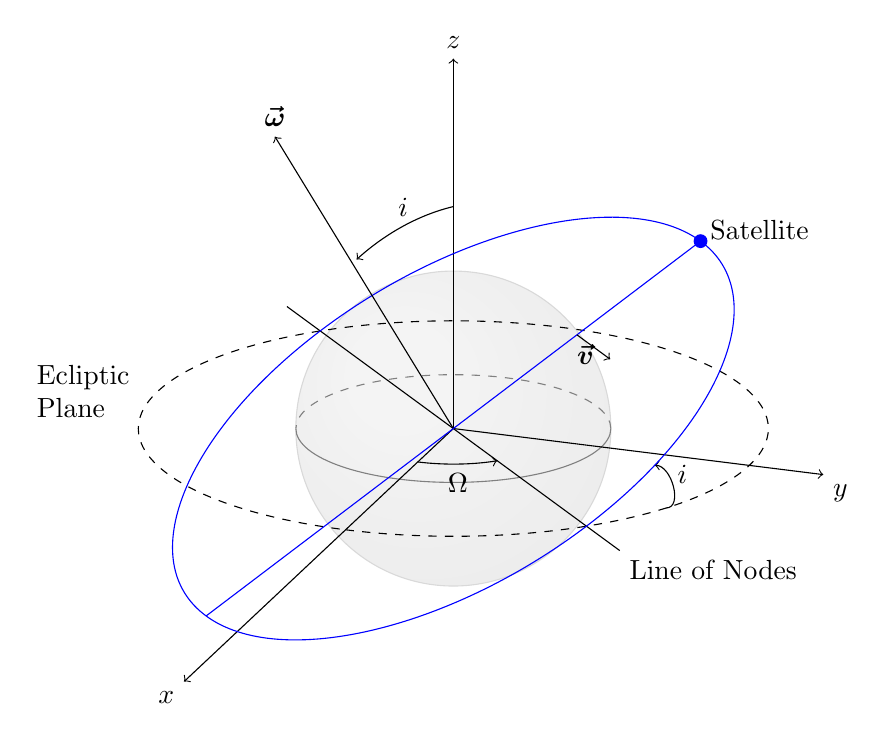
\begin{tikzpicture}[scale=5]
  \pgfmathsetmacro{\r}{.8}
  \pgfmathsetmacro{\O}{45} % right ascension of ascending node [deg]
  \pgfmathsetmacro{\i}{30} % inclination [deg]
  \pgfmathsetmacro{\f}{35} % true anomaly [deg]

  \coordinate (O) at (0,0,0);

  \pgfmathsetmacro{\Re}{0.4}
  \fill[ball color=gray!10, opacity=0.045] (0,0,0) circle ({\Re}); % 3D lighting effect
  \tdplotsetmaincoords{70}{110}
  \begin{scope}[tdplot_main_coords, shift={(0,0)}]

    % ball perimeter, gray
    \pgfmathsetmacro{\thetavec}{70}
    \pgfmathsetmacro{\phivec}{20}
    \tdplotsetrotatedcoords{\phivec}{\thetavec}{0}
    \tdplotdrawarc[tdplot_rotated_coords,color=gray!30]{(O)}{\Re}{0}{360}{}{}

    % equator
    \pgfmathsetmacro{\thetavec}{0}
    \pgfmathsetmacro{\phivec}{0}
    \tdplotsetrotatedcoords{\phivec}{\thetavec}{0}
    \tdplotdrawarc[tdplot_rotated_coords,color=black!50]{(O)}{\Re}{-70}{110}{}{}
    \tdplotdrawarc[tdplot_rotated_coords,color=black!50, dashed]{(O)}{\Re}{110}{290}{}{}

    \draw [->] (O) -- (2,0,0) node[anchor=north east] {$x$};
    \draw [->] (O) -- (0,1,0) node[anchor=north west] {$y$};
    \draw [->] (O) -- (0,0,1) node[anchor=south] {$z$};

    \node at (0,-\r,0) [left,text width=4em] {Ecliptic Plane};

    \tdplotdrawarc[dashed]{(O)}{\r}{0}{360}{}{}

    \tdplotsetrotatedcoords{\O}{0}{0}

    \draw [tdplot_rotated_coords] (-1,0,0) -- (1,0,0) node [below right] {Line of Nodes};
    \tdplotdrawarc[->]{(O)}{.33*\r}{0}{\O}{anchor=north}{$\Omega$}

    \tdplotsetrotatedcoords{-\O}{\i}{0}
    \pgfmathsetmacro{\alpha}{62.5}
    \pgfmathsetmacro{\p}{45}
    \path ({\r * cos(\alpha)},{\r * sin(\alpha)},{0}) coordinate (I1);
    \path[tdplot_rotated_coords] ({\r * cos(\alpha+\p)},{\r * sin(\alpha+\p)},{0}) coordinate (I2);
    \draw[->] (I1) to[out=360,in=0] node[pos=0.7,right] {$i$} (I2);
    \tdplotdrawarc[tdplot_rotated_coords,color=blue]{(O)}{\r}{0}{360}{}{} 
 
    \begin{scope}[tdplot_rotated_coords]
      \draw[->] (O) -- (0,0,1) node [above] {$\bm{\vec{\omega}}$};
      \draw[color=blue] (-\r,0,0) -- (\r,0,0);
      \fill[color=blue] (-\r,0,0) circle (0.5pt);
      \node[yshift=4pt,right] at (-\r,0,0) {Satellite};
      %\fill (-\r,0,0) circle[color=blue,radius=0.5pt] \node {Satellite};
      \coordinate (P) at (180:\Re);
      %\draw (O) -- (P);
      %\tdplotdrawarc[->]{(O)}{.33*\r}{180}{180+\f}{anchor=south west}{$\nu$}
    \end{scope}

    \tdplotsetrotatedcoords{-\O}{\i}{0}
    \tdplotsetrotatedcoordsorigin{(P)}
    \begin{scope}[tdplot_rotated_coords,scale=.2]
      %\draw [->] (P) -- (-1,0,0) node [right] {$\hat{r}$};
      \draw [->] (P) -- (0,1,0) node [pos=0.8,left] {$\bm{\vec{v}}$};
      %\draw [->] (P) -- (0,0,1) node [above] {$\hat{k}$};
      
    \end{scope}

  \end{scope}

  \tdplotsetthetaplanecoords{-\f}
  \tdplotdrawarc[tdplot_rotated_coords,->]{(O)}{.75*\r}{0}{\i}{anchor=south}{$i$} % not accurate :(
\end{tikzpicture}

  \caption{Geometry of a circular Earth orbit.}
  \label{fig-orbit-geometry}
\end{figure}

On the other hand, the beam movement is primarily driven by the motion of the receiving satellite in orbit, which is in turn governed by Kepler's laws of orbital motion.
Tracking capability of the aircraft can be evaluated by analysing the velocity of the sub-satellite point at the eavesdropper's operational altitude (point x on figure \ref{fig-orbit-geometry}).
If this velocity exceeds the cruise speed of the eavesdropper, the airborne platform is not able to continuously follow the uplink RF beam, which limits the time window into individual satellite passes.

\subsubsection{Equatorial orbits}

Communication satellites reside often in circular orbits, which are a special case when evaluating Kepler's laws of orbital motion.
Here, the velocity of the sub-satellite point can be computed by solving Kepler's third law for the orbital velocity at a set altitude.
In equatorial orbits, Earth's rotation can be directly substracted from the angular velocity of the satellite, as both share roughly the same rotational axis.

In essence, the aircraft can be modeled as a low-flying athmospheric satellite.
This allows for the same equations to be used in modeling its kinematic characteristics.
Solving the required velocity for successful beam tracking can be computed by equating the required orbital period of the aircraft to the one of the space-borne satellite.

Orbital period is related to the angular velocity of the satellite $\omega_{sat}$ through the equation

\begin{equation} \label{eq-ang-vel-1}
  \omega_{sat} = \frac{2\pi}{T}
\end{equation}

\noindent
which can be used to solve the tangential velocity component at a set altitude $v_r$

\begin{equation} \label{eq-ang-vel-2}
  v_r = \omega r
\end{equation}

\noindent
As $\omega_{sat} = \omega_{air}$ in the case that the aircraft is able to continuosly track the satellite, the velocity of the sub-satellite point at the cruising altitude of the aircraft $v_{r, air}$ can be solved by combining equations (\ref{eq-kepler-3}), (\ref{eq-ang-vel-1}) and (\ref{eq-ang-vel-2}).
Rearranging Kepler's third law to solve for $v_{r, air}$ gives

\begin{equation} \label{eq-v-air-equatorial}
  v_{r, air} = r_{air} \sqrt{\frac{G M_E}{r_{sat}^3}}
\end{equation}

\noindent
Variables $r_{air}$ and $r_{sat}$ are the orbital radiuses of the eavesdropping aircraft and the receiving satellite measured from the center of the Earth while $M_E$ is the mass of the Earth.
Equation (\ref{eq-v-air-equatorial}) gives $v_{r, air}$ in the ECI coordinate frame.
To compute the actual movement of the sub-satellite point relative to the surface of the Earth, the velocity figure needs to be converted to the ECF coordinate system.
For circular equatorial orbits, this can be simply achieved by substracting the spin of the Earth from $v_{r, air}$.

\begin{equation}
  v_{r, ECF} = v_{r, air} - \omega_E r_{air}
\end{equation}

\noindent
$\omega_E$ is the angular velocity of the Earth at the equator.

\subsubsection{Generalisation to inclined orbits}

Circular equatorial orbits are a good starting point for listening window analysis but their real world applications are somewhat in limited when considering relationship of orbital altitude to coverage and latency.
As discussed in section \ref{sect-orbits} and visualised in table \ref{table-megaconstellation-characteristics}, modern satellite megaconstellations aim to achieve worldwide coverage by placing a number of satellites into inclined circular Earth orbits.
Common configurations include the Walker Star and Delta constellation configurations, the advantages and disadvantages of which are discussed in more detail in the aforementioned chapter.

The same analysis methods remain valid for inclined orbits but some additional factors need to be considered.
Equatorial orbits have only a single velocity component parallel to the xy-plane in both ECI and ECF coordinate frames.
On the other hand, any inclination induces additional velocity component perpendicular to this original equatorial component.
This velocity component is visualised by $v_z$ in figure \ref{fig-inclined-v-components}.

Transitioning from the simple scalar representation into a vector space makes analyzing inclined orbital motion less cumbersome.
Here, angular velocity is a very useful abstraction, as it allows to sum different rotational speed components together.
As angular velocity does not vary in in circular motion, examining the magnitude of the sum of the angular velocity vectors allows us to gauge the tracking potential of differently inclined orbits at the desired range of altitudes.

The ECI coordinate frame is a natural starting point for evaluating orbital motion.
Angular velocity pseudovector of a circular orbit follows the right hand rule, being perpendicular to the rotational plane.
Rotational motion in the equatorial plane can be represented with angular velocity pseudovector $\bm{\vec{\omega}} = [0,0,\omega]^T$.
Inclined orbits can be generated by rotating this equatorial orbit about its diameter, which can be achieved with multiplying the pseudovector with a suitable three-dimensional rotational matrix.
To rotate the orbits about the y-axis of the ECI coordinate frame by $\theta$ degrees, rotation matrix $\bm{R_y}$ can be used.

\begin{equation*}
  \bm{R_y}(\theta) = \begin{bmatrix}
    \cos \theta & -\sin \theta & 0 \\[3pt]
    \sin \theta &  \cos \theta & 0 \\[3pt]
    0           &  0           & 1 \\
    \end{bmatrix}
\end{equation*}

Multiplying the vector by matrix $\bm{R_y}(\theta)$ and substracting the rotation vector of the Earth gives angular velocity vector in the ECF coordinate frame.
This can be in turn be converted to the velocity of the sub-satellite by taking the norm of the angular velocity pseudovector

\begin{equation*}
  \omega_{ECF} =
  ||\bm{R_y}(\theta)\ \bm{\vec{\omega_{sat, i}}} - \bm{\vec{\omega_{E}}}||
\end{equation*}

$\omega_{ECF}$ is the scalar angular velocity of the satellite in the ECF coordinate frame.
$\bm{\vec{\omega_{sat, i}}}$ and $\bm{\vec{\omega_{E}}}$ are the angular velocity vectors of the inclined satellite orbit and the spin of the Earth.
Finally, the sub-satellite velocity figure can be solved based on the scalar angular velocity by applying equation (\ref{eq-ang-vel-2}), as the altitude of the airborne platform $h_{air}$ and the mean radius of the Earth $R_E$ are known.

\begin{equation}
  v_{air} = \omega_{ECF}\ (h_{air} + R_E)
\end{equation}

\subsection{Listening window}

Listening window is the time that an airborne eavesdropper is able to intercept the uplink RF transmission from a user terminal on the ground.
Analysing this window is somewhat more complex in terms of the model required and potential input parameters that need to be considered.
On a high level, the window is primarily influenced by the relative motion between the uplink RF beam of the terminal and the kinematic characteristics of the airborne eavesdropper.
The latter include qualities such as cruise speed, operational altitude, manoeuvrability and controllability.
They define the ability of the aircraft to keep a lock on the moving RF beam.
These are in turn defined by the characteristics of the platform, a topic discussed in more detail in section \ref{sect-aerial-platforms}.
As demonstrated by the inclination-orbital altitude analysis, aircraft kinematics have very little effect at LEO satellite altitudes ranging from hundreds to couple thousand kilometers. In practice, the great disparity between the velocities makes it possible to abstract away the movement of the aircraft and assume it to be stationary for the sake of analysis.

Assuming a stationary eavesdropper, the listening window ${t_{pass}}$ can be computed by dividing the beamwidth of the satellite terminal $\theta_{beam}$ with the angular velocity of the satellite in the ECF coordinate frame $\omega_{ECF}$.

\begin{equation}
  t_{pass} = \frac{\theta_{beam}}{\omega_{ECF}}
\end{equation}

\subsection{Listening window}

\subsubsection{Equatorial orbits}

\subsubsection{Inclined orbits}


\subsection{Link budgets}
\subsubsection{Uplink transmission}
\subsubsection{Airborne jamming}

\section{Discussion}
\subsubsection{Passive eavesdropping}
\subsubsection{Active eavesdropping}
\subsubsection{Jamming}
\subsubsection{Radiolocation}


T\"ass\"a osassa esitet\"a\"an tulokset ja vastataan tutkielman alussa
esitettyihin tutkimuskysymyksiin.
Tieteellisen kirjoitelman
arvo mitataan t\"ass\"a osassa esitettyjen tulosten perusteella.

%% Huomaa seuraavassa kappaleessa lainausmerkkien ulkopuolella piste, 
%% koska piste ei lopeta lainattua tekstinp\"atk\"a\"a.
%% Jos lainattu tekstinp\"atk\"a loppuu v\"alimerkkiin, tulee v\"alimerkki
%% lainausmerkkien sis\"alle: 
%% "Et tu, Brute?" sanoi Caesar kuollessaan.
Tutkimustuloksien merkityst\"a on aina syyt\"a arvioida ja tarkastella
kriittisesti.  Joskus tarkastelu voi olla t\"ass\"a osassa, mutta se
voidaan my\"os j\"att\"a\"a viimeiseen osaan, jolloin viimeisen osan nimeksi
tulee >>Tarkastelu>>. Tutkimustulosten merkityst\"a voi arvioida my\"os
>>Johtop\"a\"at\"okset>>-otsikon alla viimeisess\"a osassa.

T\"ass\"a osassa on syyt\"a my\"os arvioida tutkimustulosten luotettavuutta.
Jos tutkimustulosten merkityst\"a arvioidaan >>Tarkastelu>>-osassa,
voi luotettavuuden arviointi olla my\"os siell\"a.

\clearpage

\section{Conclusion}

\clearpage
%% L\"ahdeluettelo

\thesisbibliography

\bibliographystyle{ieeetran}
\bibliography{main}

%% Appendices
%% If you don't have appendices, remove \clearpage and \thesisappendix below.
\clearpage

\thesisappendix

\section{Esimerkki liitteest\"a\label{LiiteA}}

Liitteet eiv\"at ole opinn\"aytteen kannalta v\"altt\"am\"att\"omi\"a ja 
opinn\"aytteen tekij\"an on 
kirjoittamaan ryhtyess\"a\"an hyv\"a ajatella p\"arj\"a\"av\"ans\"a ilman liitteit\"a.
Kokemattomat kirjoittajat, jotka ovat huolissaan
tekstiosan pituudesta, paisuttavat turhan 
helposti liitteit\"a pit\"a\"akseen tekstiosan pituuden annetuissa rajoissa.
T\"all\"a tavalla ei synny hyv\"a\"a opinn\"aytett\"a.

Liite on itsen\"ainen kokonaisuus, vaikka se t\"aydent\"a\"akin tekstiosaa.
Liite ei siten ole pelkk\"a listaus, kuva tai taulukko, vaan 
liitteess\"a selitet\"a\"an aina sis\"all\"on laatu ja tarkoitus.

Liitteeseen voi laittaa esimerkiksi listauksia. Alla on 
listausesimerkki t\"am\"an liitteen luomisesta.

%% Verbatim-ymp\"arist\"o ei muotoile tai tavuta teksti\"a. Fontti on monospace.
%% Verbatim-ymp\"arist\"on sis\"all\"a annettuja komentoja ei LaTeX k\"asittele.
%% Vasta \end{verbatim}-komennon j\"alkeen jatketaan k\"asittely\"a.
\begin{verbatim}
	\clearpage
	\appendix
	\addcontentsline{toc}{section}{Liite A}
	\section*{Liite A}
	...
	\thispagestyle{empty}
	...
	teksti\"a
	...
	\clearpage
\end{verbatim}

Kaavojen numerointi muodostaa liitteiss\"a oman kokonaisuutensa:
\begin{align}
d \wedge A &= F, \label{liitekaava1}\\
d \wedge F &= 0. \label{liitekaava2}
\end{align}


\clearpage
\section{Toinen esimerkki liitteest\"a\label{LiiteB}}

%% Liitteiden kaavat, taulukot ja kuvat numeroidaan omana kokonaisuutenaan
%%
%% Equations, tables and figures have their own numbering in Appendices
%\renewcommand{\theequation}{B\arabic{equation}}
%\setcounter{equation}{0}  
%\renewcommand{\thefigure}{B\arabic{figure}}
%\setcounter{figure}{0}
%\renewcommand{\thetable}{B\arabic{table}}
%\setcounter{table}{0}

Liitteiss\"a voi my\"os olla kuvia, jotka
eiv\"at sovi leip\"atekstin joukkoon:
%% Ymp\"arist\"on figure parametrit htb pakottavat
%% kuvan t\"ah\"an, eik\"a LaTeX yrit\"a siirrell\"a niit\"a
%% hyv\"aksi katsomaansa paikkaan.
%% Ymp\"arist\"o\"a center voi k\"aytt\"a\"a \centering-
%% komennon sijaan
%%
%% Example of a figure, note the use of htb parameters which force
%% the figure to be inserted here
%%
Liitteiden taulukoiden numerointi on kuvien ja kaavojen kaltainen:
\begin{table}[htb]
\caption{Taulukon kuvateksti.}
\label{liitetaulukko}
\begin{center}
\fbox{
\begin{tabular}{lp{0.5\linewidth}}
9.00--9.55  & K\"aytett\"avyystestauksen tiedotustilaisuus (osanottajat
ovat saaneet s\"ahk\"opostitse valmistautumisteht\"av\"at, joten tiedotustilaisuus
voidaan pit\"a\"a lyhyen\"a).\\
9.55--10.00 & Testausalueelle siirtyminen
\end{tabular}}
\end{center}
\end{table}
Kaavojen numerointi muodostaa liitteiss\"a oman kokonaisuutensa:
\begin{align}
T_{ik} &= -p g_{ik} + w u_i u_k + \tau_{ik},  \label{liitekaava3} \\
n_i    &= n u_i + v_i.                      \label{liitekaava4}
\end{align}

\end{document}
